\documentclass{beamercours}
\title{Cours TalENS 2024-2025}
\subtitle{Malédiction, \textit{My Little Pony} et Égypte}
\author{Clément Allard \& Matthieu Boyer}
\definecolor{mint}{HTML}{9ffeb0}

\newcommand{\point}[3]{\draw (#1 -.1, #2 -.1) -- (#1 + .1, #2 + .1);
\draw (#1 +.1, #2 -.1) -- (#1 - .1, #2 + .1);
\draw (#1, #2) node[below right]{#3};}

% Styles for Refraction Figures
\definecolor{v}{HTML}{00ffff}
\tikzstyle{verre} = [draw = v, fill = v!30]
\usetikzlibrary{decorations, optics}
\usetikzlibrary{angles, patterns, quotes, calc, decorations.markings, decorations.pathmorphing}

% Styles for Optics Figures in Section 2.2
% If to reuse, should add a node as argument
\tikzset{arrow inside/.style = {postaction=decorate,decoration={markings,mark=at position .52 with \arrow{stealth}}}}
\tikzset{ray/.style={very thick, red, arrow inside}}
\tikzset{line/.style={thick, black}}
\tikzset{lined/.style={thick, black, dashed}}

\newcommand{\drawreflector}[3]{\draw[#3] (-{#1*cos(#2)}+4, -{#1*sin(#2)+4}) -- ({#1*cos(#2)+4}, {#1*sin(#2)+4})}
\newcommand{\redrawreflector}[3]{\draw[#3] (-{#1*cos(#2)}+1.5, -{#1*sin(#2)+1.5}) -- ({#1*cos(#2)+1.5}, {#1*sin(#2)+1.5})}
\newcommand{\drawscreen}[3]{\draw[#3] (-{#1*cos(#2)}+7.5, -{#1*sin(#2)+1}) -- ({#1*cos(#2)+7.5}, {#1*sin(#2)+1})}
\newcommand{\cfill}[2]{\fill[pattern = north west lines]
 (-{#1*cos(#2)}+4, -{#1*sin(#2)+4}) --
 ({#1*cos(#2)+4}, {#1*sin(#2)+4}) --
 ({#1*cos(#2)+3.8}, {#1*sin(#2)+3.8}) --
 (-{#1*cos(#2)+3.8}, -{#1*sin(#2)+3.8}) --
 (-{#1*cos(#2)+4}, -{#1*sin(#2)+4}) -- cycle}
\newcommand{\recfill}[2]{\fill[pattern = north east lines]
 (-{#1*cos(#2)}+1.5, -{#1*sin(#2)+1.5}) --
 ({#1*cos(#2)+1.5}, {#1*sin(#2)+1.5}) --
 ({#1*cos(#2)+1.3}, {#1*sin(#2)+1.3}) --
 (-{#1*cos(#2)+1.3}, -{#1*sin(#2)+1.3}) --
 (-{#1*cos(#2)+1.5}, -{#1*sin(#2)+1.5}) -- cycle}

\renewcommand*{\K}{\mathbb{K}}
\graphicspath{{./Images/}}
\usepackage[utf8]{inputenc}
\usepackage[pdftex,outline]{contour}

\begin{document}
\maketitle
\begin{frame}{Plan}\tableofcontents[sectionstyle=show]
\end{frame}

\section{Faire briller un chameau ?}
\subsection{La lumière, kézako ?}

\begin{frame}
	\frametitle{Un exemple : Doom}
    \begin{figure}
        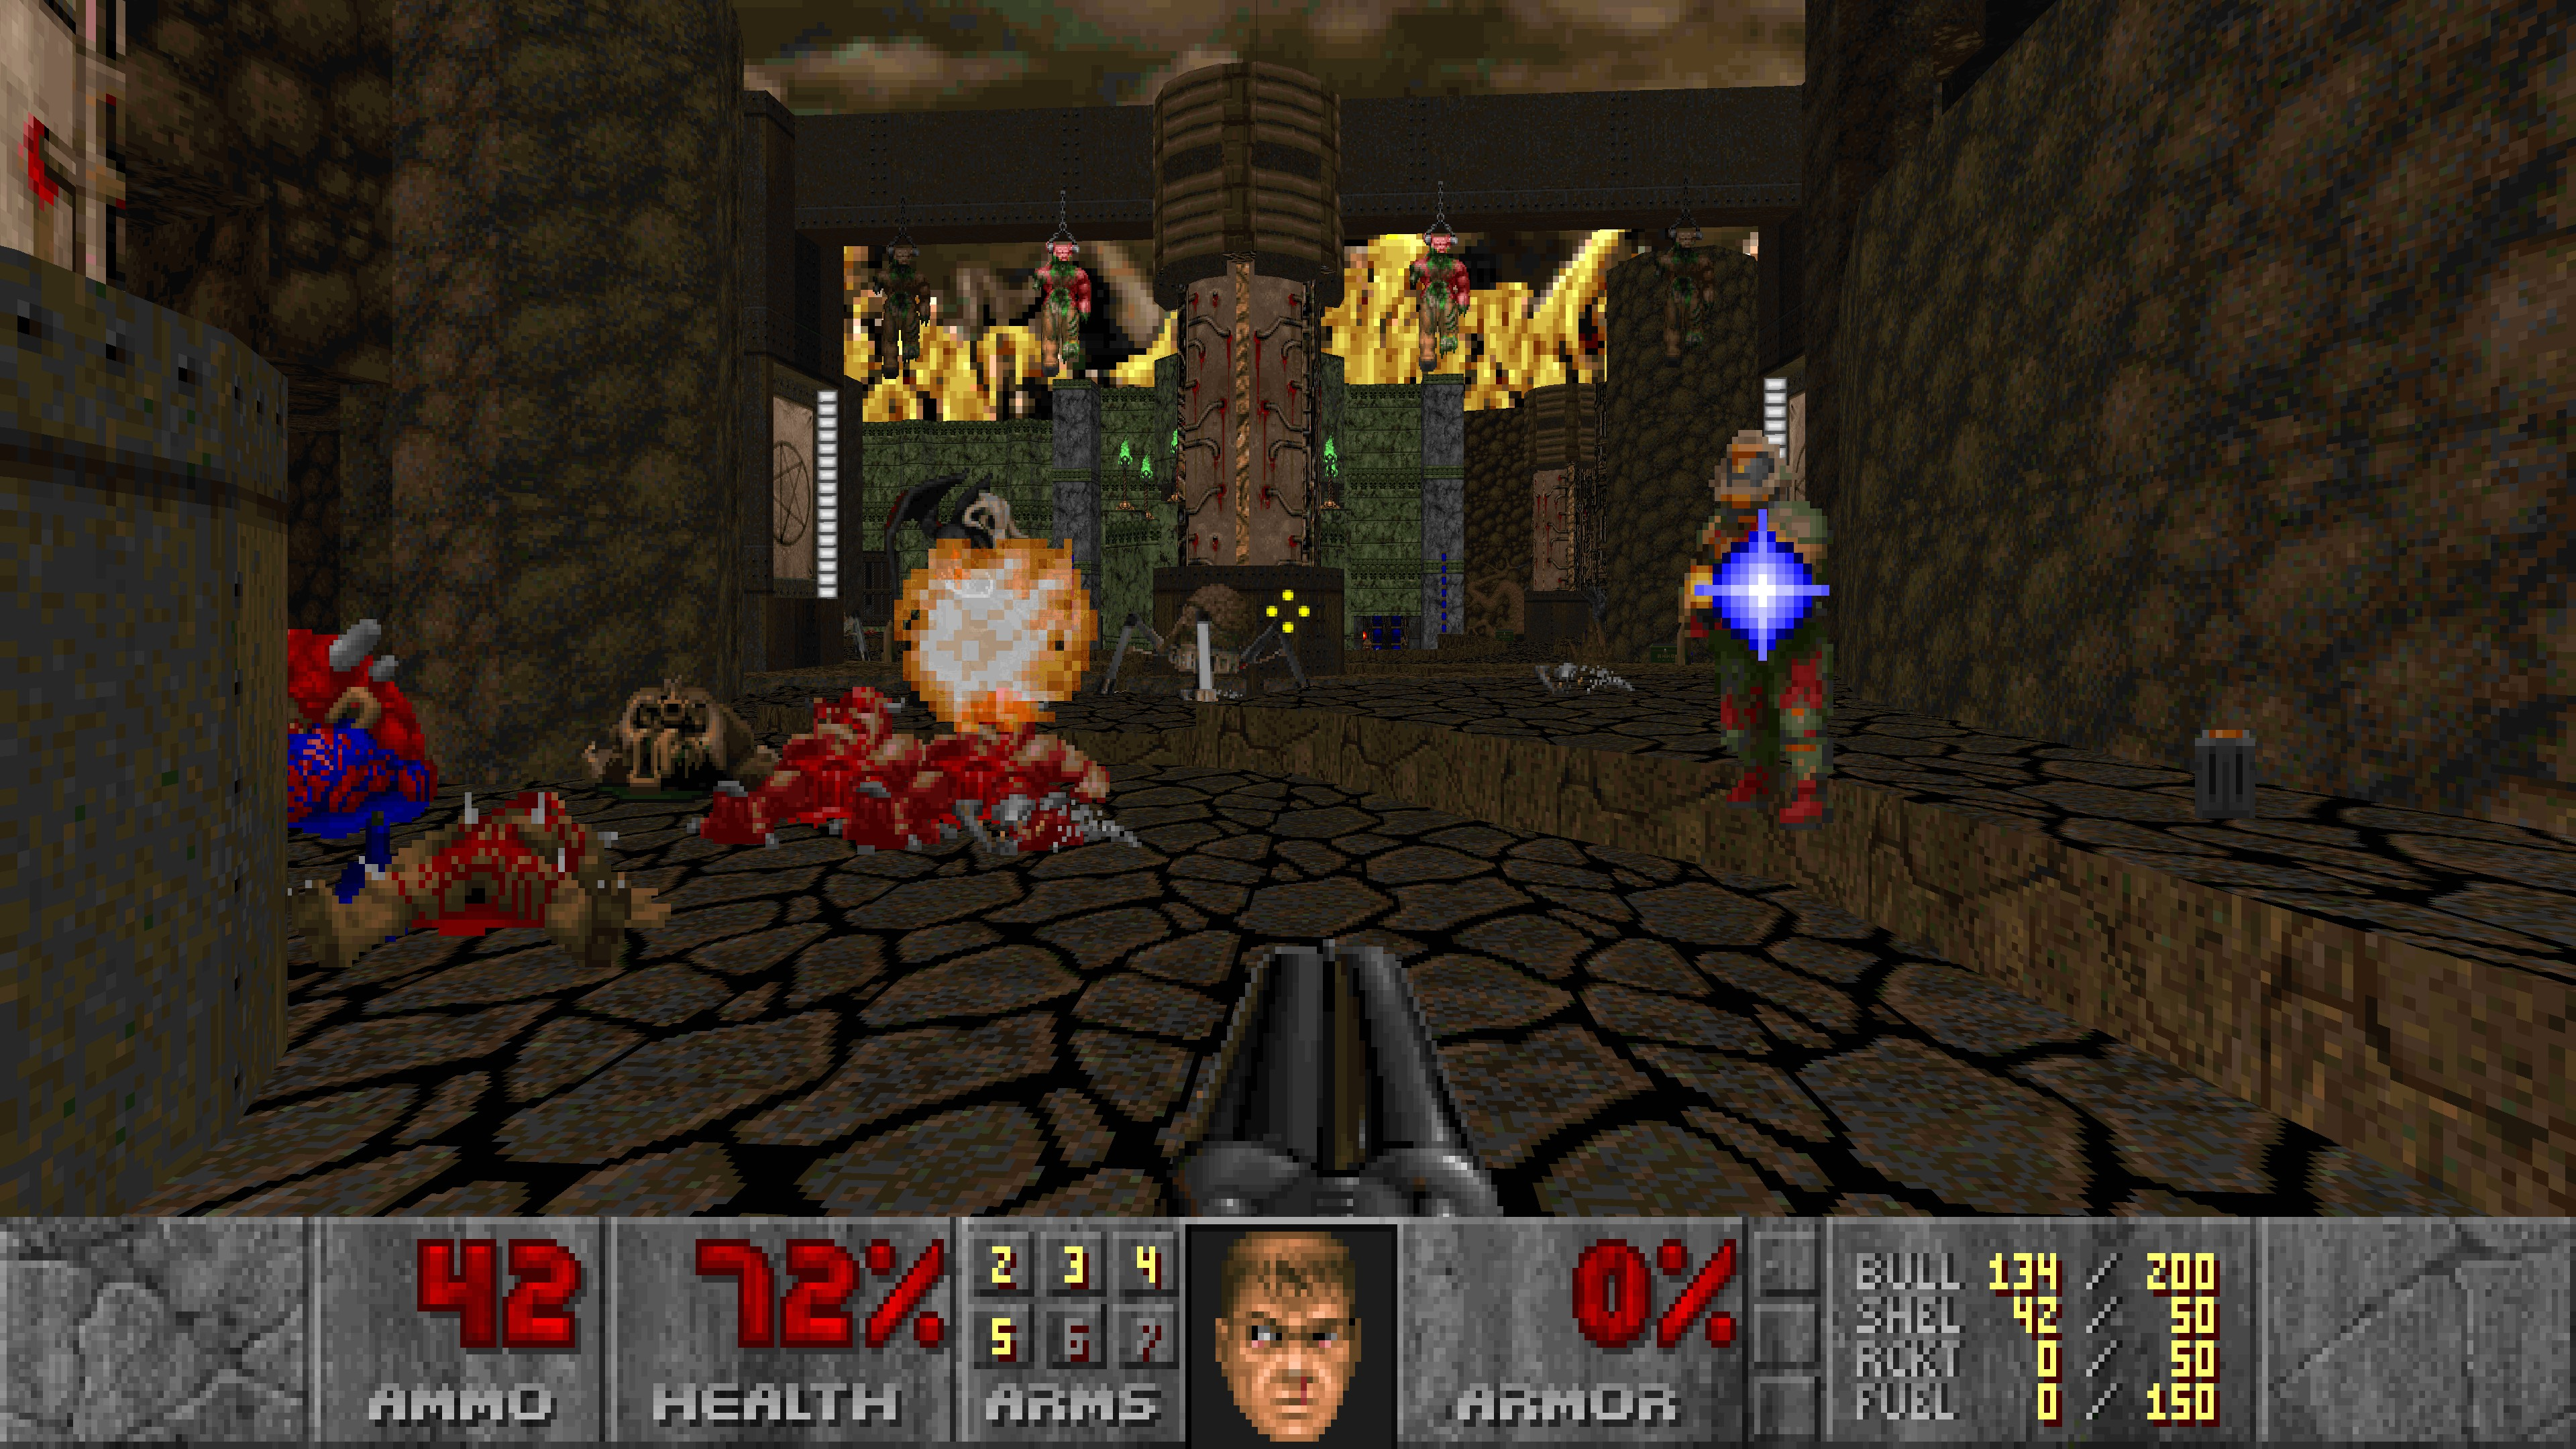
\includegraphics[scale = .07]{Doom.jpg}
        \caption{Jeu vidéo Doom}
    \end{figure}
\end{frame}

\begin{frame}
	\frametitle{Rayons lumineux}
\begin{définition}{Onde}{}
Une onde est la propagation d'une perturbation de proche en proche avec transfert d'énergie
\end{définition}

\only<2>{\begin{définition}{Rayon Lumineux}{}
On définit un rayon lumineux comme une courbe de l'espace selon laquelle se propage l'énergie lumineuse (véhiculée par l'onde électromagnétique).
\end{définition}}
\end{frame}

\begin{frame}
	\frametitle{Limites expérimentales}
	On représentera donc la lumière par des courbes fléchées, dont on ne connait pas la forme \textit{a priori}.
	\only<2>{\begin{remarque}{}{}
	D'un point de vue expérimental, la modélisation de la lumière par des rayons lumineux fonctionne bien (dans la limite d'objets assez grands devant la longueur d'onde de l'onde, pour ne pas avoir de diffraction).
	Il n'y a diffraction que dans le cas où la taille de l'objet est de l'ordre de grandeur de la longueur d'onde du rayon lumineux ($<\unit{1}{\micro\meter}$ pour les rayons visibles).
\end{remarque}}
	\only<3>{\begin{figure}[H]
	\centering
	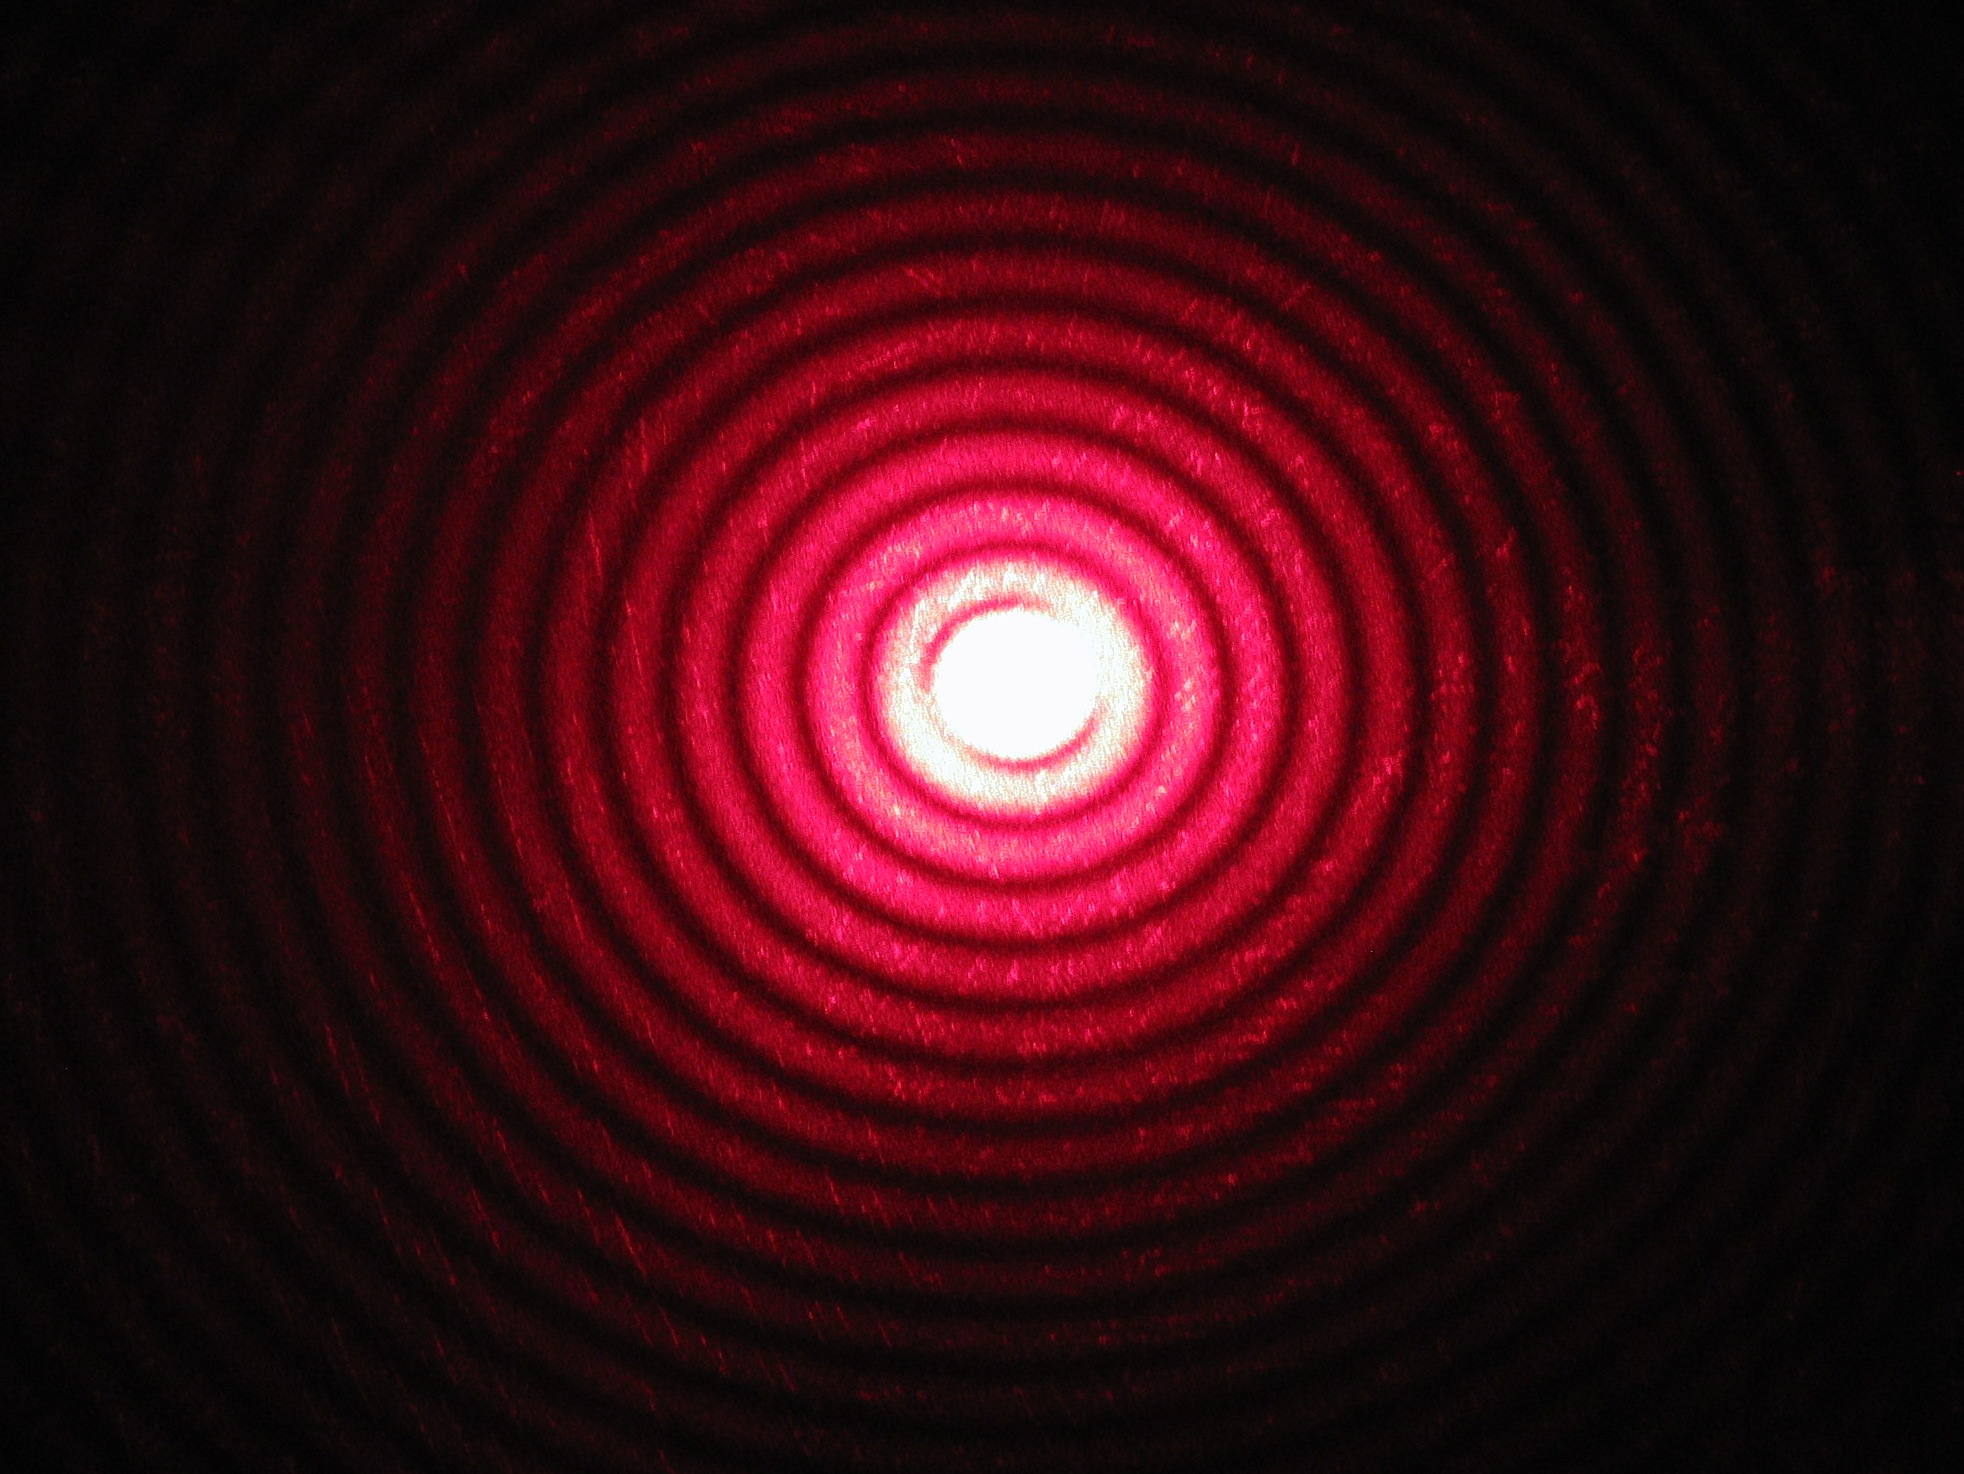
\includegraphics[scale=.08]{Diffraction.jpeg}
	\caption{Illustration du phénomène de diffraction}
\end{figure}}
\end{frame}
\subsection{Mille feux et mille couleurs}
\begin{frame}
	\frametitle{Couleurs !}
	\only<1>{\begin{définition}{Longueur d'onde}{}
	On appelle longueur d'onde d'une onde sa période spatiale $\lambda$, c'est à dire le plus petit réel non nul qui vérifie
	\begin{equation*}
		\forall x, s(x) = s(x+\lambda)
	\end{equation*}
\end{définition}}
\only<2>{
\begin{remarque}{Couleur}{}
En pratique, on peut associer à chaque longueur d'onde une couleur, comme le montre le spectre ci-dessous:
\begin{center}
	\resizebox{250pt}{!}{
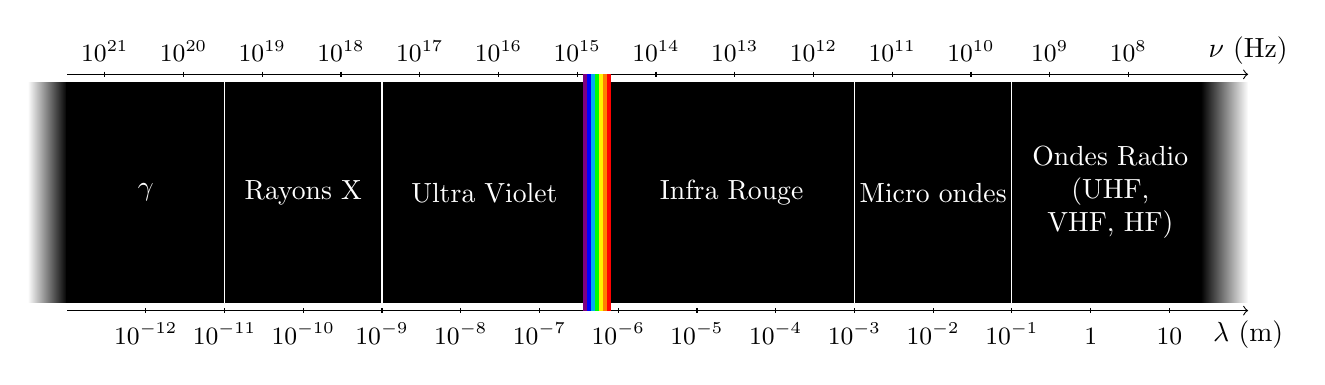
\begin{tikzpicture}[scale=1]
\shade[left color=white,right color=black] (-13.5,0.1) rectangle (-13,2.9);
\node[draw,rectangle,fill=black,text=white,minimum width=2cm,minimum height=2.8cm]  at (-12,1.5){$\gamma$};
\node[rectangle,fill=black,text=white,minimum width=2.58cm,minimum height=2.8cm]  at (-10,1.5){Rayons X};
\node[rectangle,fill=black,text width=2cm,,text=white,minimum width=2.58cm,minimum height=2.8cm,text centered] at (-7.7,1.5){Ultra Violet};
\node[rectangle,fill=black,text width=2cm,,text=white,minimum width=3.1cm,minimum height=2.8cm,text centered]  at (-4.56,1.5){Infra Rouge};
\node[rectangle,fill=black,text width=2cm,,text=white,minimum width=2cm,minimum height=2.8cm,text centered]  at (-2,1.5){Micro ondes};
\node[rectangle,fill=black,text width=2cm,,text=white,minimum width=2.5cm,minimum height=2.8cm,text centered]  at (0.25,1.5){Ondes Radio (UHF, VHF, HF)};
\shade[left color=black,right color=white] (1.4,0.1) rectangle (2,2.9);
\foreach \x in {-11,-9,-3,-1}\draw[shift={(\x,0)},thin,white] (0,3) -- (0,0);
\draw[->](-13,0)--++(15,0)node[below]{$\lambda$ (m)};
\draw[->](-13,3)--++(15,0)node[above]{$\nu$ (Hz)};
\foreach \x in{-12,-11,...,-1}
	 \draw[shift={(\x,0)}] (0pt,1pt) -- (0pt,-1pt) node[below] {\small $10^{\x}$};
\foreach \y in {21,20,...,8}
	\draw[shift={(8.48-\y,3)}] (0pt,1pt) -- (0pt,-1pt) node[above=2pt] {\small $10^{\y}$};
\foreach \x/\xtext in {1/10,0/1}
 \draw[shift={(\x,0)}] (0pt,1pt) -- (0pt,-1pt) node[below=0.2em] {\small $\xtext$};

\foreach \x/\y in {-6.42/violet,-6.37/blue,-6.32/cyan,-6.27/green,-6.22/yellow,-6.17/orange,-6.12/red}
     \draw[shift={(\x,0)},\y,line width=0.5mm] (0,3) -- (0,0);
\end{tikzpicture}}
\captionof{figure}{Spectre électromagnétique du visible}
\end{center}
\end{remarque}}
\end{frame}

\section{Comment un écran voit-il ?}
\subsection{Propagation de la lumière}

\begin{frame}
	\frametitle{MTHI et interface}
	\only<1>{\begin{définition}{MTHI - Milieux Transparents Homogènes Isotropes}{}
On s'intéresse à des milieux qui sont :
\begin{description}
	\item[Transparents:] l'énergie lumineuse n'est pas absorbée par le milieu;
	\item[Homogènes:] les propriétés du milieu ne dépendent pas du point choisi;
	\item[Isotropes:] les propriétés du milieu ne dépendent pas de la direction du rayon lumineux.
\end{description}
\end{définition}}
\only<2>{
\begin{définition}{Dioptre}{}
On appelle dioptre l'interface entre deux milieux
\end{définition}}
\end{frame}

\begin{frame}
\frametitle{Indice optique}
\begin{définition}{Indice optique}{}
On définit l'indice optique $n$ de la manière suivante
\begin{equation*}
	n=\frac{c}{v_\varphi}
\end{equation*}
où $c =\unit{299~792~458}{\meter\cdot\second^{-1}}$ est la vitesse de la lumière dans le vide et $v_\varphi$ est la vitesse de propagation de la lumière dans notre milieu.
\end{définition}
L'indice optique du vide vaut $1$, celui de l'air $1.0003$, celui de l'eau $1.33$ et le verre autour de $1.5$.
\end{frame}

\begin{frame}
\frametitle{Périodes}
\begin{remarque}{Lien période - longueur d'onde}{}
	On a ici
	\begin{equation*}
		v_\varphi = \frac{\lambda}{T}
	\end{equation*}
	où $T$ est la période temporelle de l'onde
\end{remarque}
\end{frame}

\begin{frame}
\frametitle{Lumière dans un MTHI (1)}
\begin{théorème}{Propagation de la lumière dans les MTHI}{}
	\begin{itemize}
		\item Les rayons lumineux sont des droites.
		\item Les rayons lumineux se propagent indépendamment entre eux.
	\end{itemize}
\end{théorème}
\begin{proof}
	On prouvera un de ces points ultérieurement.
\end{proof}
\end{frame}
\begin{frame}
\frametitle{Lumière dans un MTHI (2)}
\begin{propositionfr}{Droite Paramétrée}{}
	Une droite de l'espace euclidien $\R^{n}$ peut être vue comme un vecteur de norme $1$ $v \in \R^{n}$ appelé vecteur directeur associé à un point $p \in \R^{n}$ par lequel elle passe.
\end{propositionfr}
\end{frame}
\begin{frame}
\frametitle{Lumière dans un MTHI (3) : Retour inverse}
\begin{théorème}{Principe du retour inverse de la lumière}{}
Dans un MTHI, le trajet de la lumière ne dépend pas du sens de parcours
\end{théorème}
\begin{proof}
	Ceci s'illustre car le milieu est homogène et isotrope.
\end{proof}
\end{frame}

\subsection{Principe du Ray Tracing}

\begin{frame}
\frametitle{Règles du jeu}
\begin{itemize}
\item Considérons une lampe qui éclaire notre chameau. On va s'intéresser à la manière dont un observateur extérieur peut voir le chameau.
\item Un observateur extérieur ne voit une surface que si celle-ci réfléchit la lumière vers son \oe il.
\end{itemize}
\end{frame}

\begin{frame}
\frametitle{Idée naïve}
L'idée naïve est de choisir un pixel de l'écran, et de déduire la marche des rayons lumineux qui l'atteignent.
\begin{figure}[H]
	\centering
	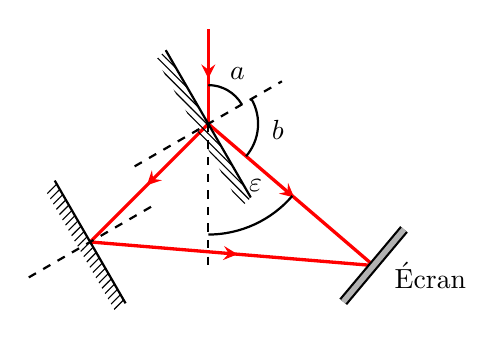
\begin{tikzpicture}[scale=.6]
		% Coordinates
		\coordinate (O) at (4,4);
		\coordinate (P) at (4,6);
		\coordinate (P') at (4,1);
		\coordinate (A) at (7.5,1);
		\coordinate (D) at (1.5,1.5);
		\coordinate (G) at ({4+3*cos(120)},{4+3*sin(120)});
		\coordinate (G') at ({4-3*cos(120)},{4-3*sin(120)});
		\coordinate (K) at ({4+3*cos(30)},{4+3*sin(30)});
		\coordinate (K') at ({4-3*cos(30)},{4-3*sin(30)});

		% Rays
		\draw[ray] (P) -- (O);
		\draw[ray] (O) -- (A);
		\draw[ray] (O) -- (D);
		\draw[ray] (D) -- (A);
		%% Dashed
		\draw[lined] (O) -- (P');

		% Reflectors
		\drawreflector{1.8}{120}{line};
		\cfill{1.8}{120};
		\drawreflector{1.8}{30}{lined};

		\redrawreflector{1.5}{120}{line};
		\recfill{1.5}{120};
		\redrawreflector{1.5}{30}{lined};

		% Angles
		\pic[draw, thick, angle radius=14pt, angle eccentricity=1.5pt, "$a$"] {angle=K--O--P};
				\pic[draw, thick, angle radius=18pt, angle eccentricity=1.4pt, "$b$"] {angle=A--O--K};
		\pic[draw, thick, angle radius=40pt, angle eccentricity=1.5pt] {angle=P'--O--A};
		\node at (5,2.7) {$\varepsilon$};

		% Viewing Screen
		\drawscreen{1}{50}{line, black, double distance = 2pt, double = black!30};
		\node at (8.7, .8) {Écran};
	\end{tikzpicture}
	\caption{Principe du Ray Tracing: trouver les rayons qui atteignent un point précis.}
\end{figure}
\end{frame}
\begin{frame}
\frametitle{Problème}
Le problème ici est qu'on doit tracer la marche d'un grand nombre de rayons pour avoir une image de bonne résolution, sachant que la plupart des rayons n'atteindront jamais l'observateur~!
\begin{figure}[H]
	\centering
	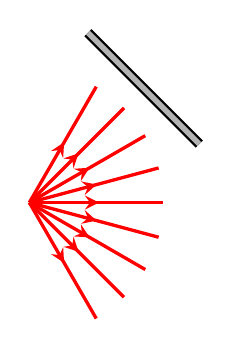
\begin{tikzpicture}
		\coordinate (O) at (0, 0);
		\coordinate (S) at (1.41, 1.41);
		\foreach \i in {-60, -45,...,60} { \draw[ray] (O) -- ({1.7*cos(\i)}, {1.7*sin(\i)}); }
		\draw[line, black, double distance = 2pt, double = black!30] (-{1*cos(135)}+1.451, -{1*sin(135)+1.451}) -- ({1*cos(135)+1.451}, {1*sin(135)+1.451});
	\end{tikzpicture}
	\caption{Rayons Passant par un Point}
\end{figure}
\end{frame}

\begin{frame}
\frametitle{Solution !}
\begin{figure}
	\centering
	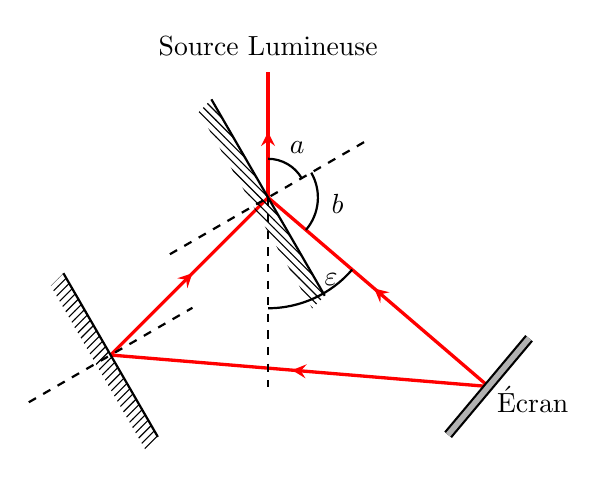
\begin{tikzpicture}[scale=.8]
		% Coordinates
		\coordinate (O) at (4,4);
		\coordinate (P) at (4,6);
		\coordinate (P') at (4,1);
		\coordinate (A) at (7.5,1);
		\coordinate (D) at (1.5,1.5);
		\coordinate (K) at ({4+3*cos(30)},{4+3*sin(30)});

		% Rays
		\draw[ray] (O) -- (P);
		\draw[ray] (A) -- (O);
		\draw[ray] (A) -- (D);
		\draw[ray] (D) -- (O);
		%% Dashed
		\draw[lined] (O) -- (P');

		% Reflectors
		\drawreflector{1.8}{120}{line};
		\cfill{1.8}{120};
		\drawreflector{1.8}{30}{lined};

		\redrawreflector{1.5}{120}{line};
		\recfill{1.5}{120};
		\redrawreflector{1.5}{30}{lined};

		% Angles
		\pic[draw, thick, angle radius=14pt, angle eccentricity=1.5pt, "$a$"] {angle=K--O--P};
				\pic[draw, thick, angle radius=18pt, angle eccentricity=1.4pt, "$b$"] {angle=A--O--K};
		\pic[draw, thick, angle radius=40pt, angle eccentricity=1.5pt] {angle=P'--O--A};
		\node at (5,2.7) {$\varepsilon$};

		% Viewing Screen
		\drawscreen{1}{50}{line, black, double distance = 2pt, double = black!30};
		\node at (8.2, .8) {Écran};
		\node at ($(P) + (0, .4)$) {Source Lumineuse};
	\end{tikzpicture}
	\caption{PRIL: La source est l'écran, l'écran est la source.}
\end{figure}
\end{frame}

\begin{frame}
\frametitle{Morale}
L'avantage : on peut se restreindre à un nombre de rayons plus limité, en ne prenant que ceux qui vont entrer dans le champ de vision de l'observateur et économisant énormément de puissance de calcul (ce qui est nécessaire pour la fluidité d'un jeu vidéo par exemple).
\end{frame}
\begin{frame}
\frametitle{Enjeux et objectifs}
Donc, pour calculer la répartition de lumière sur l'écran (et donc la couleur de chaque pixel), il nous reste à:
\begin{enumerate}
	\item Trouver comment la trajectoire d'un rayon est modifiée en rencontrant un objet.
	\item Trouver comment la couleur d'un rayon est modifiée en rencontrant un objet.
	\item Trouver comment modéliser un objet et calculer son intersection avec des rayons lumineux.
\end{enumerate}
\end{frame}

\section{Implémentation pratique}
\subsection{Prédire la lumière ?}

\begin{frame}
\frametitle{Règle fondamentale}
\begin{théorème}{Principe de Fermat}{}
La lumière se propage en minimisant son temps de parcours.
\end{théorème}
\only<2>{\begin{remarque}{}{}
Ce principe n'est pas exclusif à la lumière, et par exemple est aussi vrai pour le son (et généralement tout comportement ondulatoire) : on peut donc faire des équivalents de ray tracing sur du son ou autres.
\end{remarque}{}{}}
\end{frame}

\begin{frame}
\frametitle{Rayons lumineux et droites}
On note $(AB) = nAB$ le chemin optique. Le principe de Fermat s'écrit de manière équivalente en la minimisation du chemin optique.\\
\begin{remarque}{}{}
	Dans un milieu d'indice constant, la minimisation du chemin optique est équivalente à celle de la distance entre deux points. On sait que le chemin le plus court entre deux points est la ligne droite : on retrouve que dans un MTHI, les rayons lumineux sont des droites.
\end{remarque}
\end{frame}

\begin{frame}
\frametitle{Snell-Descartes (1)}
À l'interface entre deux milieux d'indice optique $n_1$ et $n_2$, la propagation d'un rayon lumineux en provenance du milieu $1$ se fait selon les lois suivantes :\\
\color{vulm}{Plan d'incidence :}\ \color{black} Il existe un rayon réfléchi (qui reste dans le milieu $1$) et un rayon réfracté (qui se propage dans le milieu $2$) qui sont tous les deux situés dans le plan formé par le rayon incident et la normale au dioptre.
\end{frame}
\begin{frame}
\frametitle{Snell-Descartes (2)}
\begin{tabular}{m{.3\linewidth}m{.6\linewidth}}
    Loi de la Réfraction :
    \[
        n_{1}\sin{\left(i_{1}\right)} = n_{2}\sin{\left(i_{2}\right)}
    \]
     &
    \begin{tikzpicture}[scale=1,x={(-0.353cm,-0.353cm)}, y={(1cm,0cm)}, z={(0cm,1cm)},>=stealth]
        \coordinate (O) at (0, 0, 0);
        \coordinate (A) at (2,2,0);
        \coordinate (M) at (3,4,0);
        \coordinate (B) at (2,2,-2);
        \draw[verre] (O) -- ++(4, 0, 0) ;
        \draw[verre] (O) -- +(0, 4, 0) ;
        \draw[verre](O) --++(4,0,0)--++(0,4,0)--++(-4,0,0)--cycle;
        \draw[verre](0,4,0) --++(0,0,-2)--++(4,0,0)--++(0,0,2)--cycle;
        \draw[verre](4,0,0) --++(0,0,-2)--++(0,4,0)--++(0,0,2)--cycle;
        \draw[vulm](4,2,-2)--++(0,0,4)--++(-4,0,0)--++(0,0,-4)--cycle;
        \draw[vulm] (4,2,-2) node[rotate=45,below right]{\small \hspace{10pt}Plan d'Incidence};
        \draw[dashed, vulm] (A) ++(2,0,0)--++(-4, 0, 0) ;
        \draw[->,thick,postaction={decorate},red] (4,2,1.5)--(A);
        \draw[->,thick,postaction={decorate},red] (A)--(0.4,2,-2);
        \draw[dashed, vulm, ->] (B)--++(0,0,4.5)node[below left, fill = none]{\small Normale};%la normale
        \draw[vulm] (2,2,0.5) to[bend right, vulm] (2.65,2,0.5);
        \draw (2.55,2,0.8) node[vulm]{$i_{1}$};
        \draw[vulm] (2,2,-0.5) to[bend right, vulm] (1.5,2,-0.6);
        \draw (1.55,2,-0.8) node[vulm]{$i_{2}$};
        \draw (2,0,1) node[vulm]{Indice $n_{1}$};
        \draw (2,0,-2) node[vulm]{Indice $n_{2}$};
    \end{tikzpicture}
\end{tabular}
\end{frame}
\begin{frame}
\frametitle{Snell-Descartes (3)}
\begin{tabular}{m{.3\linewidth}m{.6\linewidth}}
    Loi de la Réflexion:
    \[
        i_{1} = -i_{1}'
    \]
     &
    \begin{tikzpicture}[scale=1,x={(-0.353cm,-0.353cm)}, y={(1cm,0cm)}, z={(0cm,1cm)},>=stealth]
        \coordinate (O) at (0, 0, 0);
        \coordinate (A) at (2,2,0);
        \coordinate (M) at (3,4,0);
        \coordinate (B) at (2,2,-2);
        \draw[verre] (O) -- ++(4, 0, 0) ;
        \draw[verre] (O) -- +(0, 4, 0) ;
        \draw[verre](O) --++(4,0,0)--++(0,4,0)--++(-4,0,0)--cycle;
        \draw[verre](0,4,0) --++(0,0,-0.5)--++(4,0,0)--++(0,0,0.5)--cycle;
        \draw[verre](4,0,0) --++(0,0,-0.5)--++(0,4,0)--++(0,0,0.5)--cycle;
        \draw[vulm](4,2,-2)--++(0,0,4)--++(-4,0,0)--++(0,0,-4)--cycle;
        \draw[vulm] (4,2,-2) node[rotate=45,below right]{\small Plan d'Incidence};
        \draw[dashed, vulm] (A) ++(2,0,0)--++(-4, 0, 0) ;
        \draw[->,thick,postaction={decorate},red] (4,2,1.5)--(A);
        \draw[->,thick,postaction={decorate},red] (A)--(0,2,1.5);
        \draw[dashed, vulm, ->] (B)--++(0,0,4.5)node[above,fill=none]{\small Normale\hspace{12pt}};%la normale
        \draw[vulm] (2,2,0.5) to[bend right] (2.65,2,0.5);
        \draw (2.55,2,0.8) node[vulm]{$i_{1}$};
        \draw[vulm] (2,2,0.75) to[bend left] (1.25,2,0.6);
        \draw (1.55,2,0.9) node[vulm]{$i'_{1}$};
        \draw (2,0,1) node[vulm]{Indice $n_{1}$};
        \draw (2,0,-1) node[vulm]{Indice $n_{2}$};
    \end{tikzpicture}
\end{tabular}
\end{frame}

\begin{frame}
\frametitle{Normale}
\begin{remarque}{}{}
	Pour un objet suffisamment agréable (donc modélisable par une fonction mathématique simple $z = f(x, y)$), la normale au point $(x, y, z)$ est définie par $(-\frac{\partial{f}}{\partial{x}}, -\frac{\partial{f}}{\partial{y}}, 1)$
\end{remarque}
\end{frame}
\begin{frame}
\frametitle{Produit vectoriel}
\only<1>{\begin{définition}{Produit Vectoriel}{}
	Si $u, v \in \R^{3}$, on définit le produit vectoriel $u \times v$ de $u$ et $v$ comme le vecteur orthogonal à $u$ et $v$, de norme $\norm{u}·\norm{v}·\sin(\hat{u, v})$ et orienté selon la règle de la main droite:
	\begin{equation*}
		u \times v = \begin{pmatrix}
			u_{2}v_{3} - u_{3}v_{2}\\
			u_{3}v_{1} - u_{1}v_{3}\\
			u_{1}v_{2} - u_{2}v_{1}
		\end{pmatrix}
	\end{equation*}
\end{définition}}

\only<2>{\begin{remarque}{}{}
	Il est impossible de définir des opérateurs similaires aux produits vectoriels en dimensions supérieures. Sauf en dimension 7.
\end{remarque}}
\end{frame}

\begin{frame}
\frametitle{Triangle}
Dans le cas d'un triangle dont on connaît les trois côtés, on peut aisément trouver la normale en tout point appartenant à la face:
\begin{propositionfr}{Normale à un Triangle}{}
	Si $T = (i, j, k)$ est une face d'une triangulation de sommets $x_{i}, x_{j}, x_{k}$, alors la normale à l'objet en tout point de la face $T$ est définie par:
	\begin{equation*}
		(x_{j} - x_{i}) \times (x_{k} - x_{i})
	\end{equation*}
\end{propositionfr}
\end{frame}

\begin{frame}
\frametitle{Snell-Descartes Vecteurs Édition}
\resizebox{300pt}{!}{\begin{propositionfr}{Lois de Snell-Descartes Vectorielles}{}
	On se donne $\overrightarrow{l}$ un vecteur directeur de rayon de lumière, $\vec{n}$ la normale à la surface au point où elle est atteinte.
	On garde les notations précédentes:
	\begin{description}
		\item[Réfraction] On a:
			\vspace{-12pt}
			\begin{equation}
				\vec{v}_{\textrm{réfracté}} = \frac{n_{1}}{n_{2}}\vec{l} + \left(\frac{n_{1}}{n_{2}}\cos i_{1} - \cos i_{2}\right) \vec{n}
				\label{snelldescartesrefraction}
			\end{equation}
		\item[Réflexion] On a:
			\vspace{-12pt}
			\begin{equation}
				\vec{v}_{\textrm{réfléchi}} = \vec{l} + 2\cos i_{1}\vec{n}
				\label{snelldescartesreflexion}
			\end{equation}
	\end{description}
\end{propositionfr}}
\end{frame}

\subsection{La pouissance}

\begin{frame}
\frametitle{Coefficients}
\begin{définition}{Coefficients de puissance}{}
		\color{vulm} Coefficient en réflexion \color{black} On définit le coefficient de réflexion en puissance $R$ comme le rapport de la puissance véhiculée par l'onde réfléchie sur celle de l'onde incidente.

\end{définition}
\only<2>{On définit de même les coefficients de transmission (pour l'onde réfractée) et d'absorption (pour l'onde absorbée)}
\end{frame}

\begin{frame}
\frametitle{Conservation de la puissance (1)}
\begin{remarque}{Conservation de la puissance ?}{}
	Un objet opaque a un coefficient de transmission nul.
	Dans un MTHI, il n'y pas d'absorption de la lumière donc $A = 0$ et $R + T = 1$ (ce qui traduit la conservation de la puissance).
	Dans le cas contraire, par exemple pour un objet opaque, on a $R + T < 1$.
\end{remarque}
\end{frame}
\begin{frame}
\frametitle{Conservation de la puissance (2)}
\begin{figure}[H]
\centering
	\begin{minipage}[c]{.6\textwidth}
		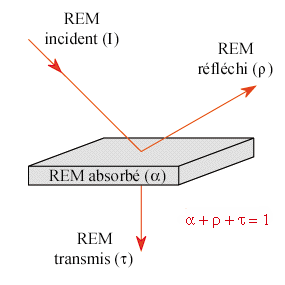
\includegraphics[width=\linewidth]{BilanRadiatif}
	\end{minipage}
	\begin{minipage}{.1\textwidth}

	\end{minipage}
	\begin{minipage}[c]{.3\textwidth}
		\caption{Bilan radiatif}
	\end{minipage}
\end{figure}

\end{frame}

\begin{frame}
\frametitle{La puissance au service de la couleur}
En pratique, on peut relier les coefficients d'absorption et de transmission aux longueurs d'ondes et donc aux couleurs. Dans le cadre d'un dioptre, on a :
	\begin{equation*}
		\begin{array}{cc}
			R = \left(\frac{n_1-n_2}{n_1+n_2}\right)^2 & T = \frac{4n_1n_2}{(n_1+n_2)^2}
		\end{array}
	\end{equation*}
La loi de Cauchy donne $n(\lambda) = A + \frac{B}{\lambda^2}$ : on a donc un lien entre la connaissance des coefficients de réflexion/réfraction et la couleur du rayon.
\end{frame}
\begin{frame}
\frametitle{Tout est bien qui finit bien}
Il suffit donc de savoir la direction initiale d'un rayon et les représentations de tous les objets dans l'environnement pour pouvoir calculer la trajectoire complète d'un rayon.
\end{frame}

\subsection{Le Chameau et l'Espace}

\begin{frame}
\frametitle{Chameau triangulé}
\begin{figure}[h]
\centering
\begin{tikzpicture}
	\begin{axis}[axis equal, scale=2, axis lines = none]
		\addplot3 [patch] file {Images/camel.dat};
	\end{axis}
\end{tikzpicture}
\caption{Triangulation d'un Chameau}
\label{fig:camel}
\end{figure}
\end{frame}

\begin{frame}
\frametitle{Triangulation : tutoriel}
\begin{définition}{Triangulation 3D}{}
	Une triangulation d'un objet est un ensemble $\mathcal{V} = \onen{n}$ de sommets ($x_{i} \in \R^{3}$ pour $i \in \mathcal{V}$), et un ensemble $\mathcal{F} \subseteq \mathcal{V}^{3 * m}$ de triangles appelés faces.
\end{définition}

Ceci nous permet de définir un objet en ne connaissant qu'un nombre fini de point.
Ceci ne change rien en réalité puisqu'on reste limité par la précision des calculs sur les nombres flottants (à virgule).
\end{frame}

\begin{frame}
\frametitle{Triangulation pour les nerds}
\begin{remarque}{}{}
	Formellement (plus ou moins), une triangulation est un complexe simplicial (ensemble de triangles) homéomorphe (qui peut être déformé sans créer de trous ni fermer de trous) à la variété (l'objet).
\end{remarque}
\end{frame}

\begin{frame}
\frametitle{Triangle et rayon :...}
On suppose donne un rayon (paramétré par $t$) $P(t) = O+ t\cdot D$ et on cherche un $t_{i}$ tel que $P(t_{i}) \in F = (P_{0}, P_{1}, P_{2})$.
On note $N$ la normale du triangle $F$.
On calcule d'abord le point d'intersection entre le rayon et le plan qui contient le triangle:
\begin{equation*}
	t_{intersect} = \frac{\left(d - N\cdot O\right)}{N \cdot D}
\end{equation*}
\end{frame}
\begin{frame}
\frametitle{...ils ne furent plus qu'un...}
On vérifie alors si le point $I = P(t_{i})$ obtenu appartient au triangle. Pour cela on calcule les coordonnées dites barycentrique $\beta_{i}$ du point (i.e. $I = \beta_{0}P_{0} + \beta_{1}P_{1} + \beta_{2}P_{2}$):
\begin{equation*}
	\beta_{i} = \norm{\left(P_{i + 2} - P_{i + 1}\right) \times \left(I - P_{i + 1}\right)}/\norm{N}
\end{equation*}
Alors $I$ est dans le triangle si et seulement si les trois $\beta_{i}$ sont entre $0$ et $1$.
\end{frame}

\begin{frame}
\frametitle{... vécurent heureux...}
\begin{algorithm}[H]
	\scriptsize
	\caption{Ray Tracing}
	\begin{algorithmic}
		\Function{\tt ray\_cast}{r, scène, profondeur}
			\If {prodondeur $>$ profondeur\_max}
			\State {couleur $\gets$ noir}
				\Else
				\If {intersection(r, scène)}
					\State {p $\gets$ point\_intersection(r, scène)}
					\State {u $\gets$ réfléchi(r, p)}
					\State {v $\gets$ réfracté(r, p)}
					\State {couleur $\gets \left(\begin{aligned}k_{R} &\times \texttt{ray\_cast}(\text{u, scène, profondeur} + 1) \\
							&+ k_{T}\times \texttt{ray\_cast}(\text{v, scène, profondeur} + 1)\end{aligned}\right)$}
				\EndIf
			\EndIf
		\EndFunction
	\end{algorithmic}
\end{algorithm}
\end{frame}

\begin{frame}
\frametitle{... et eurent beaucoup d'enfants}
Dans la vraie vie, pour se faciliter la vie, on ne va pas tester tous les points d'intersection: si on en a trouvé un on s'arrête, et on va séparer l'espace en plusieurs parties pour restreindre les objets qui pourraient potentiellement être atteints.
Toutefois, les algorithmes qui effectuent ces répartitions sont un peu trop complexes pour être détaillés ici.
Vous pouvez vous renseigner en cherchant les constructions de \emph{BVH} et des \emph{USS, Quadtree/Octree, kd-trees, BSP-trees}.
\end{frame}

\end{document}
